\chapter{Introducción}\label{cap.introduccion}
\hspace{1cm} En este primer capítulo, antes de adentrarnos en la parte mas técnica, se va a introducir al lector de forma breve que es la robótica y más concretamente en los robots aéreos, para así poder conocer el estado actual de estos robots y como ha evolucionado en los últimos años este sector, creando un gran subapartado dentro del mundo de la aviación. Una vez entrado en este contexto y conociendo el panorama mundial de la robótica aérea nos adentraremos en la Robótica Española y focalizaremos en la robótica aérea de la Universidad Rey Juan Carlos.

\section{Robótica actual}
\hspace{1cm} La Robótica es una rama multidisciplinaria de la ingeniería y la ciencia la cual incluye partes de la ingeniería mecánica, ingeniería eléctrica, ciencias de la computación y otras. Estas tecnologías permiten desarrollar máquinas que puedan sustituir a los humanos en sus acciones mas cotidianas pero sobretodo están pensadas para ser usadas en ambientes peligrosos (detección y desactivación de bombas), procesos de manufactura (montaje en serie de coches) e incluso en ambientes donde los humanos no pueden sobrevivir (otros planetas como Marte).

\hspace{1cm} Los principios básicos que se plantearon para el correcto funcionamiento de los robots desde que esta palabra fue inventada, ambos hechos realizados por el bioquímico ruso Isaac Asimov, fueron: primero que ningún robot puede hacer daño a un ser humano, o permitir que se le haga daño por no actuar, segundo que un robot debe obedecer las órdenes dadas por un ser humano, excepto si éstas órdenes entran en conflicto con la primera ley y tercero que un robot debe proteger su propia existencia en la medida en que está protección no sea incompatible con las leyes anteriores. Todo esto actualmente, como se ha visto en la sociedad actual es muy difícil de que se cumpla y dista mucho de la realidad y, aunque si que se exigen unos mínimos a la hora de crear robots, cualquier parecido es mera casualidad.
\\
\\
\begin{figure}[H]
 \centering
  \subfloat[Robot Artificiero]{
   \label{f:Robot Artificiero}
    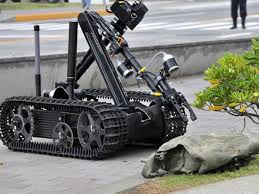
\includegraphics[width=0.33\textwidth]{imag/IMG1.jpeg}}
  \subfloat[Robots en cadena de montaje]{
   \label{f:Robots en serie de montaje}
    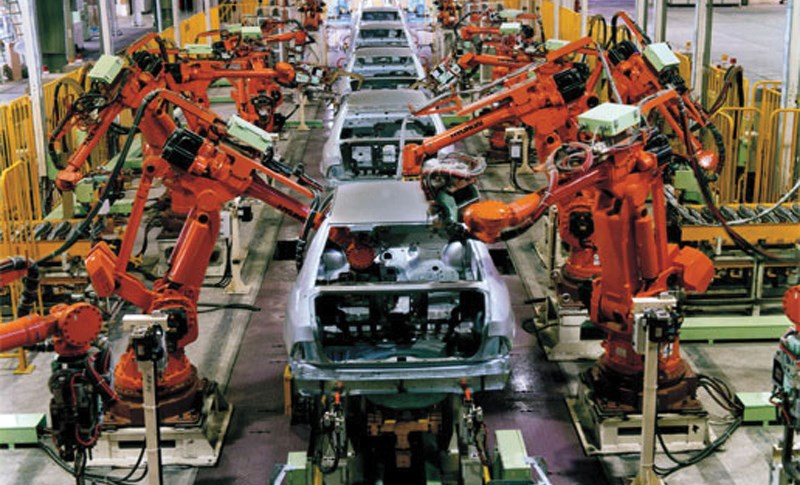
\includegraphics[width=0.33\textwidth]{imag/IMG2.jpeg}} 
  \subfloat[Rover Curiosity en Marte]{
   \newline\label{f:Rover Curiosity en Marte}
    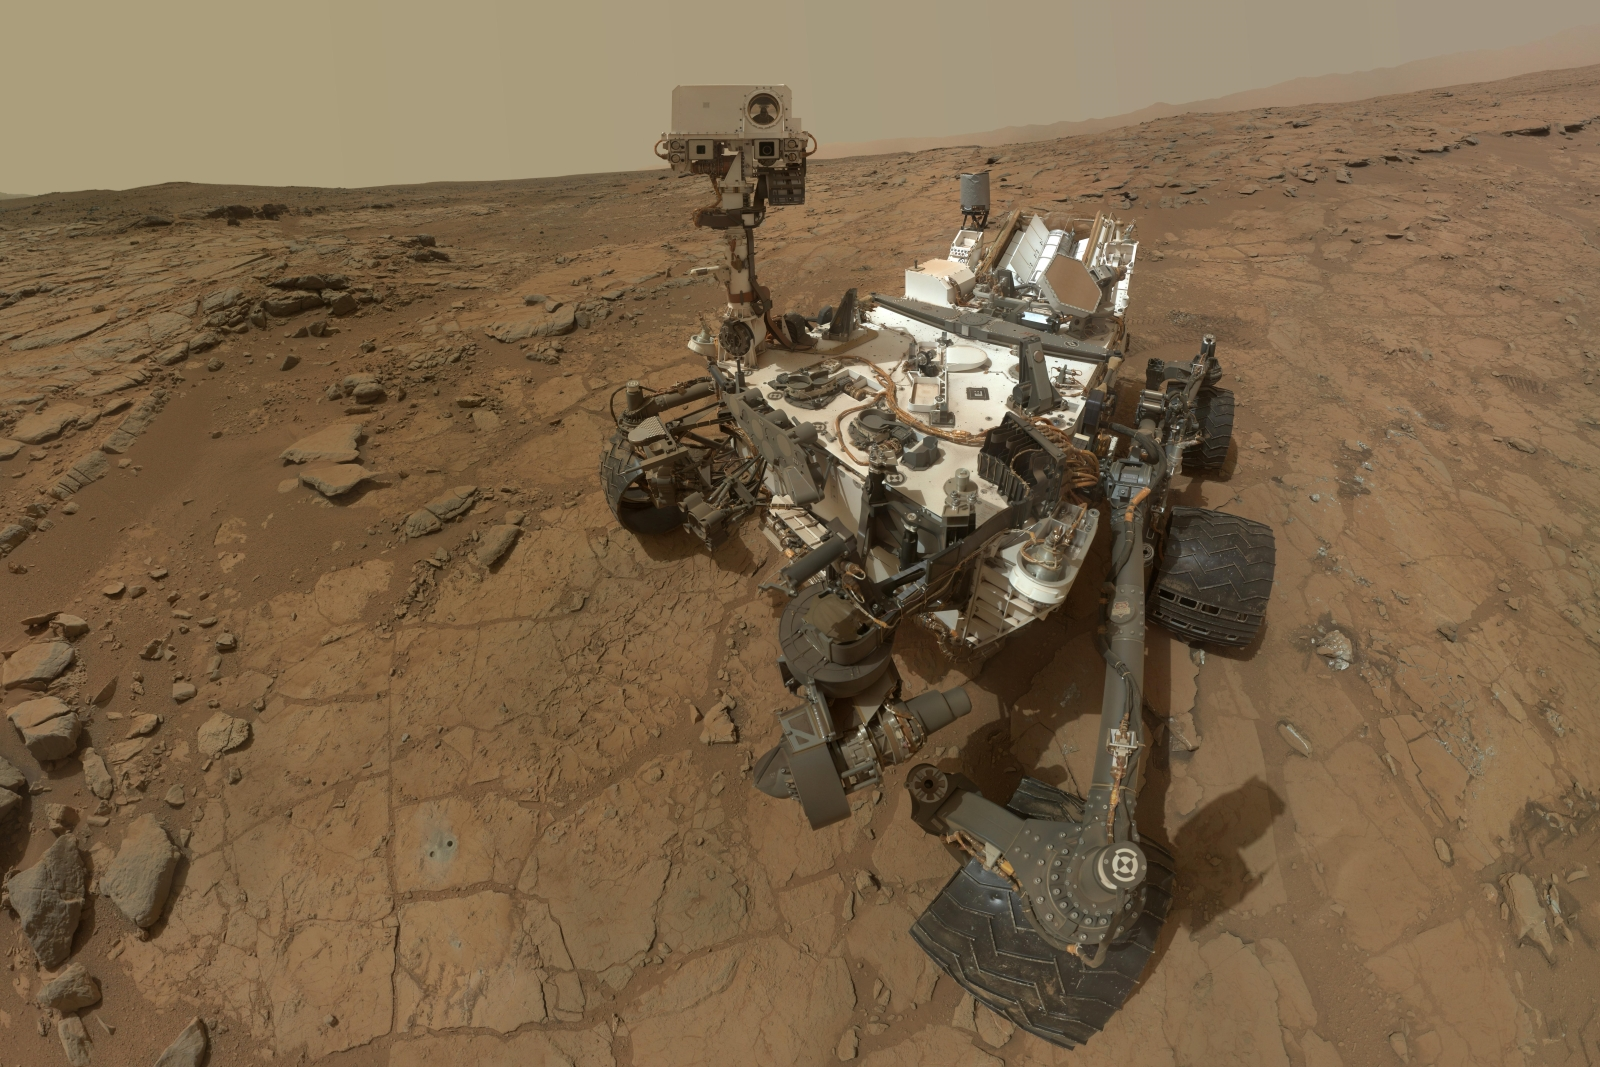
\includegraphics[width=0.33\textwidth]{imag/IMG3.jpeg}} 
 \caption{Ejemplos de funcionalidades de Robots}
 \label{f:Ejemplos de funcionalidades de Robots}
\end{figure}  

\subsection{Clasificación}
\hspace{1cm} Hay muchos tipos de clasificación de los robots, pero el mas utilizado y reconocido es según su cronología:

\begin{itemize}
		\item \textbf{1ª Generación:} Robots manipuladores. Sistemas mecánicos de varias funcionalidades con un sistema de control sencillo, el cual puede ser manual, de secuencia fija o de secuencia variable.

	\item\textbf{2ª Generación:} Robots de aprendizaje. Son capaces de repetir una secuencia de movimiento que ha sido previamente ejecutada por una persona. El operador realiza los movimientos requeridos mientras el robot los memoriza y le va siguiendo. 

	\item\textbf{3ª Generación:} Robots con control sensorizado. Llevan incorporados controladores, pequeñas computadoras que ejecutan las ordenes de un programa y mediante el manipulado es capaz de realizar los movimientos ordenados.

	\item\textbf{4ª Generación:} Robots inteligentes. Similares a la generación anterior pero incluyen una gran mejora y es que están equipados con sensores que mediante la comunicación con la computadora de control sobre la realización de las ordenes permite una toma inteligente de decisiones y un control de procesos en tiempo real.
\end{itemize}

\begin{figure}[H]
	\begin{center}
		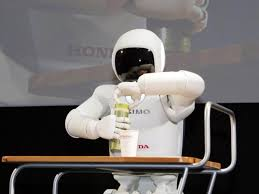
\includegraphics[width=0.5\textwidth]{imag/IMG11.jpeg}
				\caption{Robot ASIMO realizando acciones cotidianas.} 
	\label{fig:Robot ASIMO.}	
	\end{center}
\end{figure}

\hspace{1cm} Como hemos dicho anteriormente la robótica es una ciencia que esta en constante desarrollo, gracias a esto a evolucionado increíblemete en los últimos años, esto ligado al incremento de los procesadores, así como en dispositivos hardware y desarrollo de software ha permitido que hoy en día la robítica este presente en prácticamente todas las industrias actuales y cotidianas de nuestra vida:
\begin{itemize}
		\item \textbf{Agricultura: }Todavía no son muy comunes los robots que trabajan en agricultura, pero a medida que pasa el tiempo se vuelven más y más populares. La tecnología robótica aplicada al sector agrícola se encuentra en un estado de desarrollo avanzado debido a la necesidad de aumentar la producción sin aumentar los recursos al mismo tiempo que se minimiza el impacto ambiental.
		\item \textbf{Educación: }La robótica ha surgido como un recurso didáctico innovador que favorece la construcción de conceptos y conocimientos de distintas disciplinas, no únicamente las tecnológicas o científicas.  Utilizando esta tecnología como factor de motivación a partir del interés para llevar al alumno al desarrollo de su propio conocimiento.
		\begin{figure}[H]
			\begin{center}
				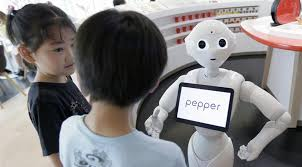
\includegraphics[width=0.9\textwidth]{imag/IMG12.jpeg}
					\caption{Robot PEPPER en un aula como complemento educador.}
			\label{fig:Robot PEPPER.}	
			\end{center}
		\end{figure}

		\item \textbf{Industria: }Se utilizan tanto para realizar trabajos peligrosos o de gran dificultad para un humano como puede ser la aplicación de sustancias nocivas, el moldeado de materiales o el transporte pesado; como para tareas de inspección y control de calidad mediante visión artificial y sistemas mecánicos. Además, el uso de robots conlleva una mejora de calidad y un gran aumento de la productividad.
		\item \textbf{Investigación: }En los laboratorios se utilizan para realizar tareas repetitivas de medición y control de calidad y desempeñar trabajos peligrosos para los humanos como puede ser la manipulación de sustancias dañinas. También en la investigación espacial se hace un gran uso de la robótica, lo que permite investigar entornos que para un ser humano serían prácticamente imposibles, como el caso del robot Curiosity mencionado anteriormente.
		\item \textbf{Medicina: }Se han desarrollado dispositivos que permiten realizar desde trabajos quirúrgicos guiados por imágenes hasta cirugía mínimamente invasiva realizada mecánicamente por un robot. También podemos encontrar robots asistenciales para personas que necesitan una supervisión y cuidado continuo, prótesis robóticas que van desde la sustitución parcial de alguna parte dañada del cuerpo hasta exoesqueletos. Otro ejemplo estaría en la robótica terapéutica, utilizada como medio de rehabilitación fisiológica y en tratamientos para enfermedades como el Alzheimer. Por último hablar de los nano-robots que son capaces de combatir por si solos diferentes enfermedades del cuerpo humano.
		\begin{figure}[H]
			\begin{center}
				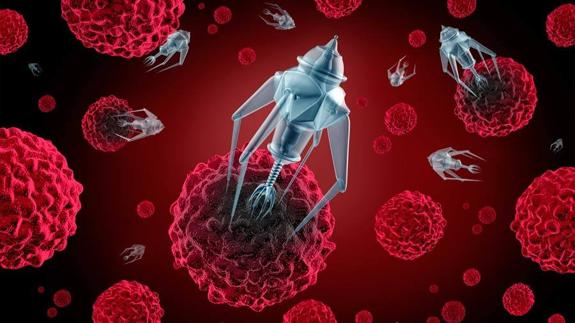
\includegraphics[width=0.7\textwidth]{imag/IMG13.jpeg}
					\caption{Nanorobots para combatir enfermedades.}
			\label{fig:Nanorobots.}	
			\end{center}
		\end{figure}	
			
		\item \textbf{Militar: }En muchas ocasiones los mayores avances en materia de tecnología se han realizado durante periodos de guerra. Actualmente existe una gran gama de vehículos terrestres sin piloto humano con funciones de reconocimiento e incluso algunos vehículos armados. El mayor desarrollo en cuanto a robótica militar está siendo llevada a cabo en la robótica aérea, donde estos sistemas han pasado de ser unidades de apoyo a unidades primarias de ataque.
		\item \textbf{Ocio y tiempo libre: }En los últimos años se ha producido una integración de esta tecnología en eventos de cultura, deporte y ocio. Podemos ver ejemplos de esto en eventos deportivos en los que se aplica la realidad aumentada, en el desarrollo de efectos especiales de la industria audiovisual o en las nuevas generaciones de consolas y videojuegos, en los que se hace amplio uso de la visión por computador. Aquí también podríamos incluir los robots para niños que son capaces de divertir y entretener a la vez, y están llegando a todos los hogares.
		\item \textbf{Seguridad: }La robótica ha dado al mundo de la seguridad y la vigilancia una nueva perspectiva, siendo la visión artificial el eje en torno al que giran estas aplicaciones. La automatización de estas tareas permite una mayor facilidad y eficiencia a la hora de ejecutar esta labor, podemos encontrar drones que vigilan grandes concentraciones de personas, cámaras en seguridad vial que analizan el tráfico o el uso doméstico de estas para la prevención de accidentes.
\end{itemize}

\subsection{Visión Artificial, Enrutamiento y Autolocalización}
\hspace{1cm} Para muchos científicos el sentido del cual el ser humano obtiene mas información del medio es la visión, de hecho, debido a esta gran cantidad de datos se calcula que el 70\% de las tareas del celebro se emplean en analizar esta información visual. Por esto la Visión Artificial o Visión por Computador busca conseguir la información visual para extraer las características que le interesan y así poder utilizar procedimientos automáticos. Para conseguir que todo esto fuese viable y no se tardara días en enviar imágenes se emplearon las técnicas de procesamiento de imágenes las cuales han avanzado a niveles de que el desfase entre la visión atificial y la realidad sea prácticamente nulo.

\begin{figure}[H]
	\begin{center}
		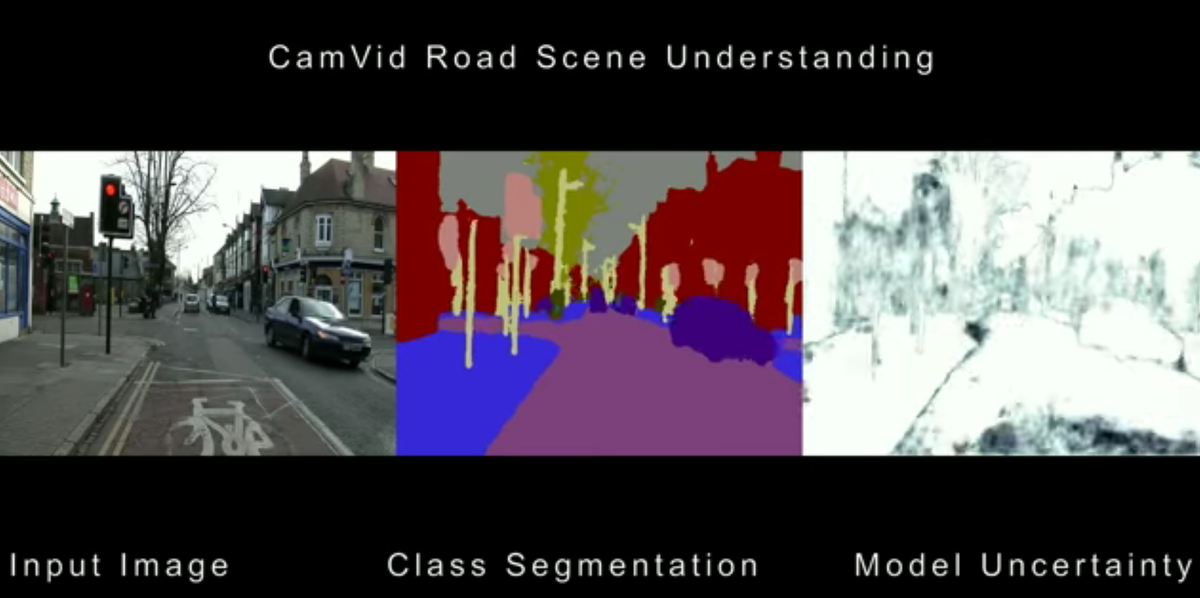
\includegraphics[width=0.9\textwidth]{imag/IMG4.png}
				\caption{Visión artificial de un automóvil.}
	\label{fig:Vista artificial automoviles.}	
	\end{center}
\end{figure}

\hspace{1cm} Para poder hablar de la Visión Artificial lo primero es conocer la naturaleza de la luz ya que esta técnica se basa en diferenciar esta para poder analizarla y enviar la información de las imágenes. Resumiendolo brevemente la luz es la parte de la radiación electromagnética que puede ser percibida por el ojo humano y la luz visible corresponde a la radiación del espectro visible, ambas están formadas por fotones cuyas propiedades en relación con la dualidad de onda explican las características de su comportamiento. Una vez conocida la naturaleza de la luz, la Visión Artificial se basa en la formación de imágenes y, como hemos dicho antes, en el sistema de procesamiento de éstas. El primer apartado estaría constituido  por  el  subsistema  de  iluminación,  de  captación  de  la  imagen  y  de adquisición  de  la  señal  en  el  computador, una vez se ha conseguido introducir la señal en el computador se procesa mediante algoritmos para transformarla en información útil para los robots.
 
\hspace{1cm} El enrutamiento es el proceso por el cual una persona o robot busca un camino entre todos los posibles, normalmente está asociado a una serie de puntos o itinerarios que debe seguir, por lo que la complegidad radica en que realice la sucesión de estos de la mejor forma posible encontrando la ruta óptima. Los parametros mas importantes a la hora del enrutamineto son la metrica y el algoritmo de cálculo.
En cuanto a la métrica es importante porque de esta de extrae el valor que luego los algoritmos utilizaran para determinar cual es la mejor ruta, hay muchos tipos de metrica, dla mas utlizada en el día a día suelen ser las longitudinales (metros, pies...), pero hay muchas mas como las temporales o las electronicas (ancho de banda, segun protocolo) utilizadas en telecomunicaciones. Por otra parte el algoritmo de cálculo es la parte mas compleja de desarrollar y sera mediante la cual obtengas la ruta optima por lo que su objetivo al final es conseguir una ruta que reduzca el retardo entre puntos de la red, consiga el mejor enlace entre puntos de ruta y por ultimo reduzca el coste de la operación.

hspace{1cm} En estos últimos años y gracias a la privación del GNSS y la utilización de este sistema para la sociedad guera de la industria militar ha permitido que hoy podamos utilizar la localización en cualquier dispositivo con una simple antena, ha su vez y visto el potencial de este sistema de autolocalizacion todos los paises han intentado crear su red satelital de posicionamiento, el primero y promotor de todo fue GPS (EE.UU.), Galileo (UE), Beidu (India), Glonass (Rusia)... Con toda esta red de satelies y la posibilidad de los nuevos softwares que permiten la utilización de varios sistemas conjuntamente, prácticamente todos los dispositivos utilizan un localizador GNSS para posicionarse, el problema viene cuando la posición que necesitamos es tridimensional y tiene que ser muy precisa, ya que este sistema aun cuenta con fallos de metros en cuantro al posicionamiento tridimensional. Por ello, en nuestro proyecto, no podremos utilizar este sistema de posicionamiento y lo cambiaremos por la autolocalización mediante balizas visuales, la cual nos dara un error mucho menor y nos permitira realizar el enrutamiento y guiado mucho mas preciso.


\section{Robótica Aérea}
\hspace{1cm} Los robots aéreos o mas comúnmente conocidos como UAV (Unmanned Aerial Vehicle), son vehículos aéreos no tripulados (VANT) controlados remotamente desde una estación de control en tierra y/o mar, o por un programa previamente implementado, estos son los llamados UAV autónomos, programados para que respondan ante el entorno e incluso interactúen con el.

\hspace{1cm} Inicialmente estos robots se pensaron unicamente para uso militar y fueron investigados y desarrollados por este sector, empezaron a crearse entre los años 1914 y 1918, durante la I Guerra Mundial, cuando estaban pensados para utilizarse como blancos aéreos de entrenamiento y defensa contra los Zeppelins, se continuaron desarrollando durante la II Guerra Mundial también para entrenar a los operarios de los cañones antiaéreos pero pronto se vio el potencial que tenían estos robots aéreos y se decidió dejar de utilizar unicamente como blanco aéreo para utilizarlo con fines mas productivos como la vigilancia, iniciada durante la guerra de Vietnam,  y la obtención, manejo y transmisión de información ya sea propia u obtenida por los mismos UAV y así poder proteger la misma de la guerra electrónica y la criptografía ya que las comunicación son mucho mas seguras y dificiles de detectar.

\hspace{1cm} Hasta este último siglo se pensaba que serian investigados unicamente para la industria militar, pero visto el gran potencial que tenían, los nuevos usos que se les estaban dando y los avances en  la industria aeronáutica e informática permitió que se convirtiese en una herramienta útil para la sociedad civil. Por tanto en la actualidad los UAV son útiles en diferentes industrias con diferentes objetivos y así una posible clasificación de los mismos sería:

\begin{itemize}
		\item \textbf{Blanco:} Fue el primer uso que se le dio a los UAV y que permitió el posterior avance y desarrollo que ha obtenido. Servían como simulación de aviones y ataque enemigos para poder entrenar las defensas de los ejércitos.
		\item\textbf{Reconocimiento:} Uso que revelo el gran potencial de estos robots, servían para enviar información militar recopilada durante el vuelo, normalmente en las zonas enemigas. 
	\begin{figure}[H]
		\begin{center}
			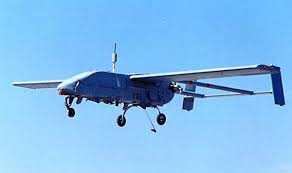
\includegraphics[width=0.7\textwidth]{imag/IMG14.jpeg}
					\caption{AAI RQ-2 Pioneer - Uno de los primeros Robots Aéreos.}
		\label{fig:UAV Pioneer.}	
		\end{center}
	\end{figure}		
		
		\item \textbf{Combate:} estos son los llamados UCAV(unmanned combat air vehicle)	usados para llevar a cabo misiones de combate que suelen ser peligrosas.
		\item \textbf{Logística:} o tambien llamados de carga, utilizados sobretodo para transportar mercancías peligrosas o sobre zonas en conflicto sin el riesgo de perder vidas humanas.
		\item \textbf{Investigación y Desarrollo:} en estos se prueban y se mejoran los sistemas que están en desarrollo para comprobar su correcto funcionamiento.
		\item \textbf{Comercial y Civil:} ultima utilización que se ha llevado a cabo y que se encuentra en mayor crecimiento tanto de innovaciones como de ventas ya que son diseñados para propósitos civiles como pueden ser: realizar filmaciones , inspección y reparaciones, sondas de investigación, rescates, vigilancia, detección de incendios y agricultura entre otros.
\end{itemize}

\hspace{1cm} La mayoría de los UAV actuales cuentan con una serie de partes, sensores y actuadores que les permiten realizar los propósitos para los que has sido creados, entre ellos encontramos: 
	\begin{itemize}
		\item \textbf{Motor:} En esta parte diferenciaremos los de ala fija los cuales se rigen por el mismo principio de vuelo que los aviones en los cuales la sustentación se produce gracias a la forma de las alas y el enfrentamiento de estas frente al viento, y los de ala rotatoria, estos se rigen por el principio de vuelo de los helicópteros en los cuales las propias hélices del motor son las que por su forma y giro porducen la sustentación y por tanto el vuelo del drone, término muy utilizado para este tipo de UAV. 		
\begin{figure}[H]
 \centering
    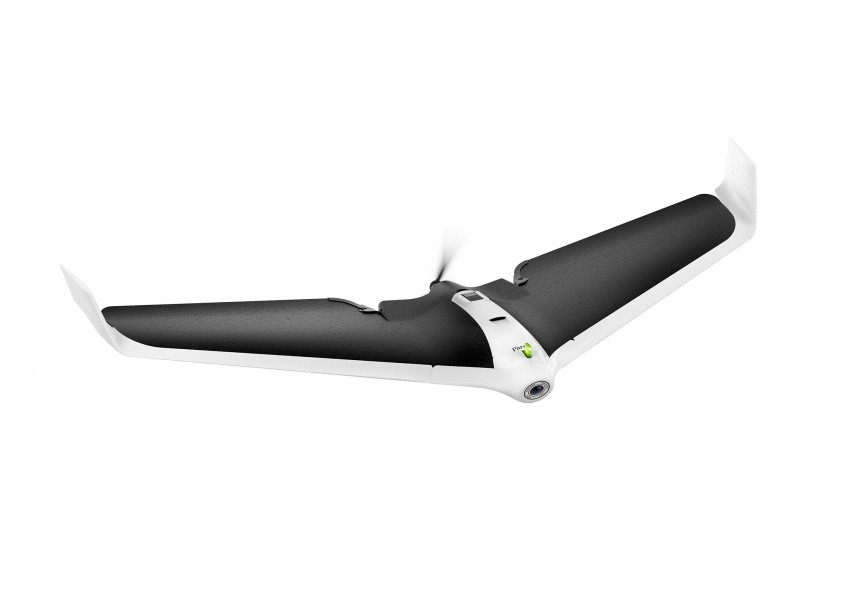
\includegraphics[width=7cm,height=4cm]{imag/IMG15.jpeg}
    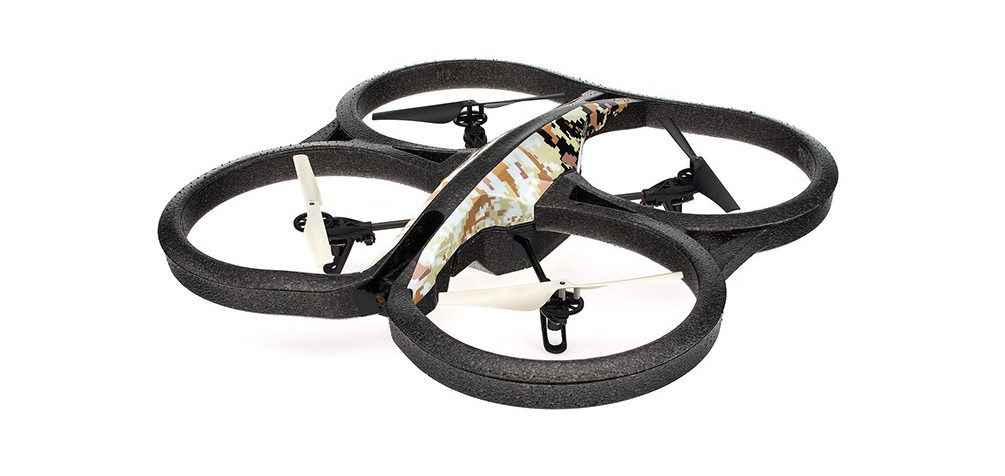
\includegraphics[width=7cm,height=4cm]{imag/IMG16.jpeg}
 \caption{Drone ala fija Vs Drone ala móvil}
 \label{f:Tipos de Drone}
\end{figure}

		\item \textbf{Chasis:}Estructura principal  sobre  la  que  se sitúan el resto de los elementos. Cambiará su forma dependiendo del tipo de UAV, variando la longitud del cuerpo de aterrizaje o el número de soportes para los motores o hélices. Gracias a los últimos avances en la ingeniería de materiales se ha conseguido que el chasis sea mucho mas ligero y así poder incrementar la carga útil(pay-load) para mejorar la funcionalidad de los mismos.
		\item \textbf{Batería:} La parte mas crítica por el momento de los UAV y en la que mas se esta investigando, la autonomía media de los UAV no supera la hora de vuelo y esto es debido a que los motores necesitan mucha potencia para poder hacer volar los drones por lo que cuanto mas grandes mas potencia es necesaria y por tanto mayor batería se necesita, por lo que hay que encontrar el término justo que se necesita para cada drone en cuanto a peso, carga útil y autonomía. 
		\item \textbf{Equipo transmisor y receptor:} Parte encargada la transformación de la información y si fuese el caso de la comunicación simultanea con el equipo en tierra. Parte muy importante para los UAV que están teledirigidos o que transmiten información simultanea de lo que están haciendo, normalmente mediante radiofrecuencia o Wi-Fi.
		\item \textbf{Controlador:} Encargado de recoger toda la información tanto de la previamente cargada como de los sensores para procesarla y ejecutar las ordenes adecuadas para completar el objetivo que se le ha establecido. 
		\item \textbf{Cámara:} Aunque no todos los UAV la llevan incorporada, es una parte imprescindible en el desarrollo de los mismos ya que permite saber en todo momento lo que está realizando el drone y poder analizar estas imágenes para comprobar el correcto funcionamiento, incluso hay UAV que únicamente se encargan de grabar una determinada zona o fotografiarla (mapeo o filmación), estos drones cuentan con varias cámaras verticales y horizontales para no perder ningún detalle y poder ver en todas las direcciones.
		\item \textbf{Altímetro:} Es el sensor que mide los cambios en la presión atmosférica de forma que puede establecer la altura a la que se encuentra el dron.
		\item \textbf{IMU:} es un dispositivo electrónico que mediante una combinación de acelerómetros y giróscopos determina la velocidad, orientación y las fuerzas gravitacionales del vehículo para comprobar el correcto funcionamiento del controlador y de los motores en cualquier entorno y condición meteorológica y en caso erróneo, los dispositivos mas avanzados, pueden corregirlo.
		\item \textbf{Magnetómetro:} es un dispositivo que mide la dirección del campo gravitacional de la tierra y de esta forma calcula la orientación del dispositivo con respecto a ésta, lo cual es muy útil para poder direccionar el dron sobre rutas terrestres.
	\end{itemize}

\hspace{1cm} Con esta breve caracterización y clasificación de los UAV nosotros nos centraremos sobretodo en los Robots Aéreos de ala móvil, concretamente en los cuadricópteros que son los que están formados por cuatro hélices las cuales permiten el movimiento en todas las direcciones posibles mediante la variación de potencia de los motores que hacen girar estas hélices. En la siguiente imagen se pueden observan como se producen los principales movimientos del dron, donde las flechas indican el sentido de rotación de las hélices y el color la velocidad del giro, el rojo significa mayor velocidad. Como diferenciación de la forma de vuelo de los helicópteros destacar que en estos la torsión generada por el rotor principal se contrarresta con una hélice de apoyo perpendicular a ésta y en los drones cuadricópteros el problema de la torsión se solventa asignando el sentido de giro de las hélices de forma opuesta entre rotores que están situados de forma contigua.

\begin{figure}[H]
 \centering
  \subfloat[Rotores en cruz +]{
   \label{f:Rotores en cruz}
    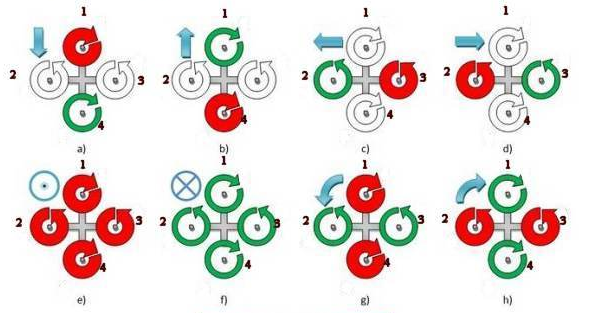
\includegraphics[width=0.53\textwidth]{imag/IMG5.png}}
  \subfloat[Rotores en aspa x]{
   \label{f:Rotores en aspa}
    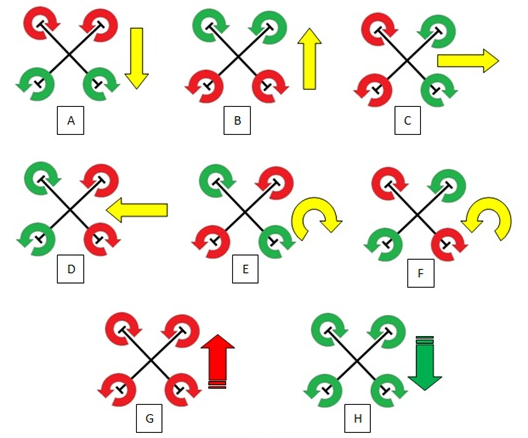
\includegraphics[width=0.38\textwidth]{imag/IMG6.png}} 
 \caption{Movimiento del Drone según sus rotores.}
 \label{f:Moviento en drones.}
\end{figure}

\subsection{Robótica aérea Española}
\hspace{1cm} En esta sección nos centraremos principalmente en el marco legislativo en España sobre los UAV, que se acordó el 15 de Diciembre de 2017 en el Consejo de Ministros \footnote{\url{https://www.boe.es/boe/dias/2017/12/29/pdfs/BOE-A-2017-15721.pdf}}, y en los avances mas importantes que se han llevado a cabo en nuestro país. 

\hspace{1cm} La nueva ley sigue cumpliendo prácticamente la totalidad de la ley aprobada el 4 de Julio de 2014 en la cual se especificaba: 
\begin{itemize}
		\item Tipo de Drone: Se establecen dos categorías iniciales: Drones con peso inferior a 2Kg. y drones con peso entre los 2Kg. y 25Kg. Para ambos es imprescindible disponer de un carnet de piloto de drones para poder operar en España. En caso de los drones de peso inferior a 2kg, no será necesario que estén inscritos en el registro de aeronaves ni disponer de un certificado de aeronavegabilidad. Para ambos tipos de drone, será necesario incluir obligatoriamente una placa identificativa con el nombre del fabricante del aparato así como los datos fiscales de la empresa que lleve a cabo dichas operaciones.
		\item Espacio aéreo: El espacio aéreo pertenece a AESA, y como tal, para poder realizar cualquier tipo de actividad comercial o civil con un drone, se deberá obtener un permiso oficial, como mínimo 5 días antes de llevar a cabo cualquier operación en el aire. Esta nueva legislación sigue manteniendo la prohibición de sobrevolar núcleos urbanos o espacios con una alta masificación de gente sin el consentimiento especial por parte de la Agencia Española de Seguridad Aérea.
		\item Seguridad: El pilar fundamental en el que se ha basado el Ministerio para la realización de la normativa de uso de drones civiles en España es la seguridad. Por ello cada empresa deberá disponer de un manual de operaciones cumplimentado siguiendo el estándar proporcionado por el Ministerio, así como un estudio de seguridad de cada una de las operaciones a realizar. Es decir, si alguien piensa en hacer volar un drone al margen de la ley, ya sea con un peso inferior a 2kg, o entre 2kg y 25kg, se expone a sanciones que van entre 3.000\textup{\euro} a 60.000\textup{\euro}.
		\item Carnet de piloto de Drones en España: Para que las empresas puedan operar legalmente, como lo hace Dronair, los pilotos designados deberán disponer de un carnet oficial para el manejo de drones.. Si estos pilotos ya disponen de un título de piloto de avión, ultraligero u otro específico, no será necesario obtener dicha titulación. En caso contrario deberán cursar una serie de exámenes y pruebas oficiales para obtener el carnet oficial de piloto de drones. A día de hoy, no existen academias oficiales bajo la tutela del Gobierno que realicen estos cursos, por eso y mientras se empiezan a impartir estos cursos, será obligatorio demostrar que se dispone de los conocimientos teóricos y algún tipo de carnet oficial o documento que acredite a los pilotos en el manejo de drones para poder llevar a cabo cualquier operación. Esta normativa temporal sobre drones en España considera los diferentes marcos en los que se podrán realizar los distintos trabajos aéreos y en función del peso de la aeronave. Además, el texto aprobado se completa con el régimen general de la Ley 48/1960, de 21 de julio, sobre Navegación Aérea, y no sólo marca las pautas de operación con este tipo de aeronaves, sino también otro tipo de obligaciones.
	\end{itemize}
	
\hspace{-1cm} Las únicas novedades de la ley puesta en marcha a finales del año pasado son:

	\begin{itemize}
		\item Sobrevolar zonas pobladas: Ésta es una de las medidas más esperadas por el sector. Se podrán realizar vuelos sobre aglomeraciones, edificios y reuniones de personal al aire libre siempre y cuando la masa máxima al despegue de la aeronave no sobrepase los 10kg, mantengamos la aeronave dentro del alcance visual del piloto (VLOS) y no sobrepasemos los 120 metros de altura ni los 100 metros en horizontal con la posición del piloto.
		\item Vuelos nocturnos: Con la actual ley 18/2014 no se permite realizar vuelos nocturnos con RPAs. Los vuelos nocturnos están recogidos en el borrador de la nueva ley y parece que van a ser permitidos siempre y cuando tengamos la autorización de la Agencia Estatal de Seguridad Aérea. Esto supone además que es necesario contar con un estudio de seguridad.
		\item Vuelos en espacio aéreo controlado: Por el momento solamente está permitido volar en zonas de espacio aéreo no controlado. Con la nueva ley se podrá volar en espacio aéreo controlado siempre y cuando presentemos los estudios de seguridad correspondiente y tengamos la autorización de AESA.
		\item Operaciones EVLOS: Con la normativa vigente solamente podemos alejar nuestra aeronave a una distancia máxima de 500 metros en horizontal respecto a la posición del piloto. Con la nueva normativa estarán permitidos los vuelos dentro del alcance visual aumentado (EVLOS). Es decir, estos 500 metros pueden ser ampliados, siempre y cuando existan observadores intermedios coordinados entre si. En todo momento, al menos uno de ellos debe tener visión directa del vehículo.
	\end{itemize}	 

\hspace{1cm} En cuanto a los inventos de drones o de usos de estos nos basaremos en los dos certamenes mas importantes tanto a nivel nacional como internacinal. A nivel internacional tenemos el Premio UAE Drones For Good Award en los Emiratos Árabes en el cual los siguientes proyectos españoles han llegado a ser finalistas: transferir rápidamente órganos de trasplantes desde los centros de donantes, vigilar mejor las zonas verdes para combatir la caza furtiva, controlar la vida salvaje y reducir el riesgo se incendios, ofrecer mejor detección de campo de minas y combatir la propagación de la enfermedad del sueño (Tse-Tse) mediante el control de mosquitos.

\begin{figure}[H]
	\begin{center}
		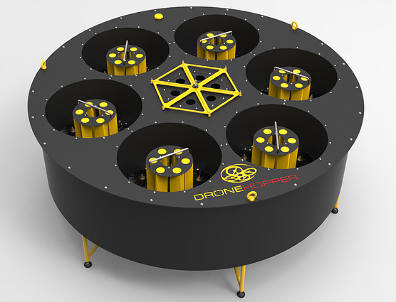
\includegraphics[width=0.5\textwidth]{imag/IMG7.jpeg}
				\caption{Dron contra incendios.} 
	\label{fig:Dron Hopper.}	
	\end{center}
\end{figure}

\hspace{1cm} A nivel nacional tenemos el Premio que se ha creado este año a la Innovación Aeronáutica por el COIAE(Colegio Oficial de Ingenieros Aeronáuticos de España) y que ha ganado dron que extingue incendios forestales, el cual tiene la capacidad de adaptarse a las condiciones de un fuego para apagarlo\footnote{\url{https://www.drone-hopper.com}}.


\subsection{Robótica áerea en la URJC}
\hspace{1cm} Proyectos anteriores en los que me he basado y que me han ayudado para crear mi trabajo de final de carrera:

\hspace{1cm} Alberto Martín: \footnote{\url{http://jderobot.org/Amartinflorido-tfm}} Navegación visual en un cuadricóptero para el seguimiento de objetos. En el abordaba la navegación visual autónoma de un cuadricóptero implementando algoritmos de navegación visual para el seguimiento de objetos de manera autónoma tanto con la camara frontal como con la cmara inferior.

\begin{figure}[H]
	\begin{center}
		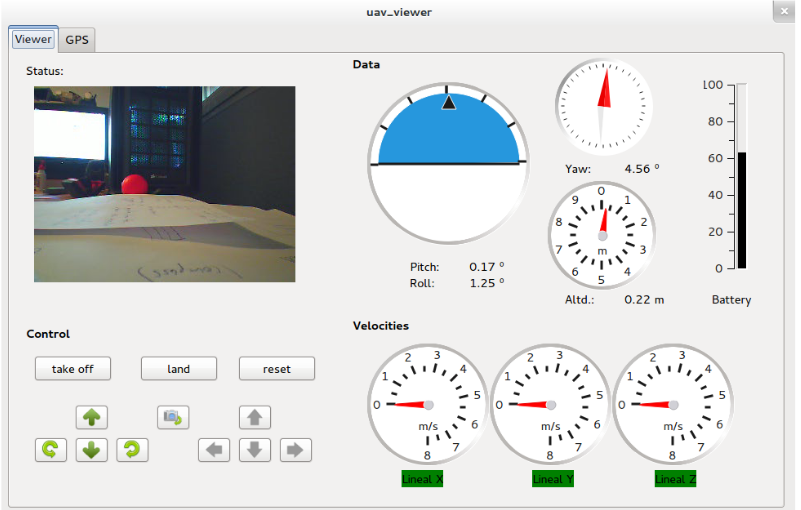
\includegraphics[width=0.7\textwidth]{imag/IMG8.png}
				\caption{TFM Alberto Martín.} 
	\label{fig:TFM Alberto M.}	
	\end{center}
\end{figure}

\hspace{1cm} Daniel Yagüe: \footnote{\url{http://jderobot.org/Daniyague-pfc}} Cuadricóptero AR.Drone en Gazebo y JdeRobot. En el cual su objetivo era proporcionar un soporte para robots aéreos en el entorno JdeRobot dentro del simulador Gazebo y crear varias aplicaciones de navegación para validarlo en entornos reales.

\hspace{1cm} Alberto López-Cerón Pinilla: \footnote{\url{http://jderobot.org/Alopezceron-tfm}} Autolocalización visual robusta basada en marcadores. Su objetivo principal era crear un algoritmo de autolocalización visual basado en marcadores, es decir , a partir de la detección de balizas. Fue creado tanto para el entorno de simulación como para entornos reales.

\hspace{1cm} Arturo Vélez: \footnote{\url{http://jderobot.org/Avelez-tfg}} Seguimiento de un objeto con textura desde un drone con
cámara. Aquí trabajó en un seguimiento visual, esta vez sin filtro de color, donde el dron sigue una textura en movimiento detectando unos puntos de interes para reconocerla.

\hspace{1cm} Manuel Zafra: \footnote{\url{http://jderobot.org/Mazafrav-pfc}} Seguimiento de rutas 3D por un drone con autolocalización
visual con balizas. Diseño un sistema de vuelo autónomo para drones en espacios interiores, basandose en la autolocalización mediante la visión artificial.

\begin{figure}[H]
 \centering
    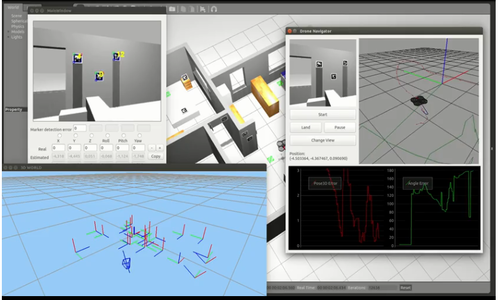
\includegraphics[width=7cm,height=4cm]{imag/IMG9.png}
    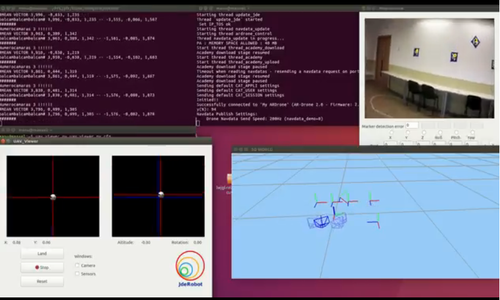
\includegraphics[width=7cm,height=4cm]{imag/IMG10.png}
 \caption{TFG Manuel Zafra.}
 \label{f:TFG Manuel Zafra}
\end{figure} 

\hspace{1cm} Jorge Vela: \footnote{\url{http://jderobot.org/Jvela-tfg}} Despegue, navegación y aterrizaje visuales de un drone usando jderobot. Se centro en la localización y aterrizaje controlado de un drone mediante la deteccion visual de balizas. 

